\chapter{Code-Reuse Technique}
\label{ssec:my-rop-chain}
%To show the feasibility of SnakeGX, we built our proof-of-concept
%on top of the research proposed by Biondo et al.~\cite{biondo2018guard}.
To show the feasibility of SnakeGX, we choose for our proof-of-concept
the technique described by Biondo et al.~\cite{biondo2018guard}.
This means that SnakeGX uses ROP. 
%\todo{FT: suggestion: "SnakeGX does not rely on a specific technical, but it 
%does require one to control its behavior."}
However, as stated in Section~\ref{sec:threat-model}, 
%SnakeGX does not require any specific code-reuse technique as long as this 
%allows controlling the enclave behaviour.
SnakeGX does not rely on a specific technique, but it does require one to 
control its behavior.
Moreover, we adapted their approach to work on the Intel SGX SDK newer versions.

In the original approach, the authors exploited \texttt{asm\_oret()} and 
\texttt{continue\_execution()} functions.
%, both described in~\cite{biondo2018guard}. %Section~\ref{ssec:cont}.
More precisely, they crafted a set of fake frame in order to create a loop between these functions.
In the x$64$ architecture, the first four function parameters are passed by registers.
Therefore, the authors used \texttt{asm\_oret()} for setting \texttt{continue\_execution()} registers pointing to a controlled structure.
However, as also Biondo underlined, it is more complicated to use 
\texttt{asm\_oret()} for SDK $2.0$.
This is why in our approach we substituted \texttt{asm\_oret()} with a 
\emph{glue gadget}.
This might be any gadget that sets the input register for the \texttt{continue\_execution()} function.
Since we developed our proof-of-concept for Linux 64bit, \texttt{continue\_execution()} expects the first argument
(\ie a \texttt{sgx\_exception\_info\_t} address) in the \texttt{rdi} register.
This is achievable by using a classic \texttt{pop rdi} gadget. 
Windows, instead, follows a different calling convention
and \texttt{continue\_execution()} expects an \texttt{ocall\_context} address shifted by $8$ byes in the \texttt{rcx} register.
Therefore we used a \texttt{pop rcx} as a \emph{glue gadget}.
In our evaluation, we found \texttt{pop rdi} and \texttt{pop 
rcx} gadgets in the Intel SGX SDK version for Linux and Windows, respectively.

Figure~\ref{fig:flavio-enclave-chain} describes our code-reuse technique.
The attacker crafts a fake stack that can reside inside or outside the enclave,
we used both approaches. The fake stack is composed by frames, one of which contains in order:
\begin{enumerate*}[label=(\roman*)]
	\item a \emph{glue gadget} address,
	\item a fake \texttt{sgx\_exception\_info\_t} address,
	\item the \texttt{continue\_execution()} address.
\end{enumerate*}
Once the first \emph{glue gadget} is triggered, it will set \texttt{rdi} (or \texttt{rcx} in Windows) register pointing to the fake \texttt{sgx\_exception\_info\_t} structure.
Then, the \texttt{continue\_execution()} will set registers according to \texttt{sgx\_exception\_info\_t} 
and it will also pivot to the actual gadget.
Since \texttt{continue\_execution()} allows us to control all general registers,
we can easily invoke another function instead of a simple gadget (\eg \texttt{memcpy} in Frame~$1$).
Finally, the gadget will return at the beginning of the next frame.
At this point, the CPU will trigger a new \emph{glue gadget} and the attack continues.

Our technique is more flexible compared to the one described by Biondo.
By using a \emph{glue gadget}, we can easily drive \texttt{continue\_execution()} without
relying on other SDK functions that might change in future versions.

\begin{figure}[t]
	\centering
	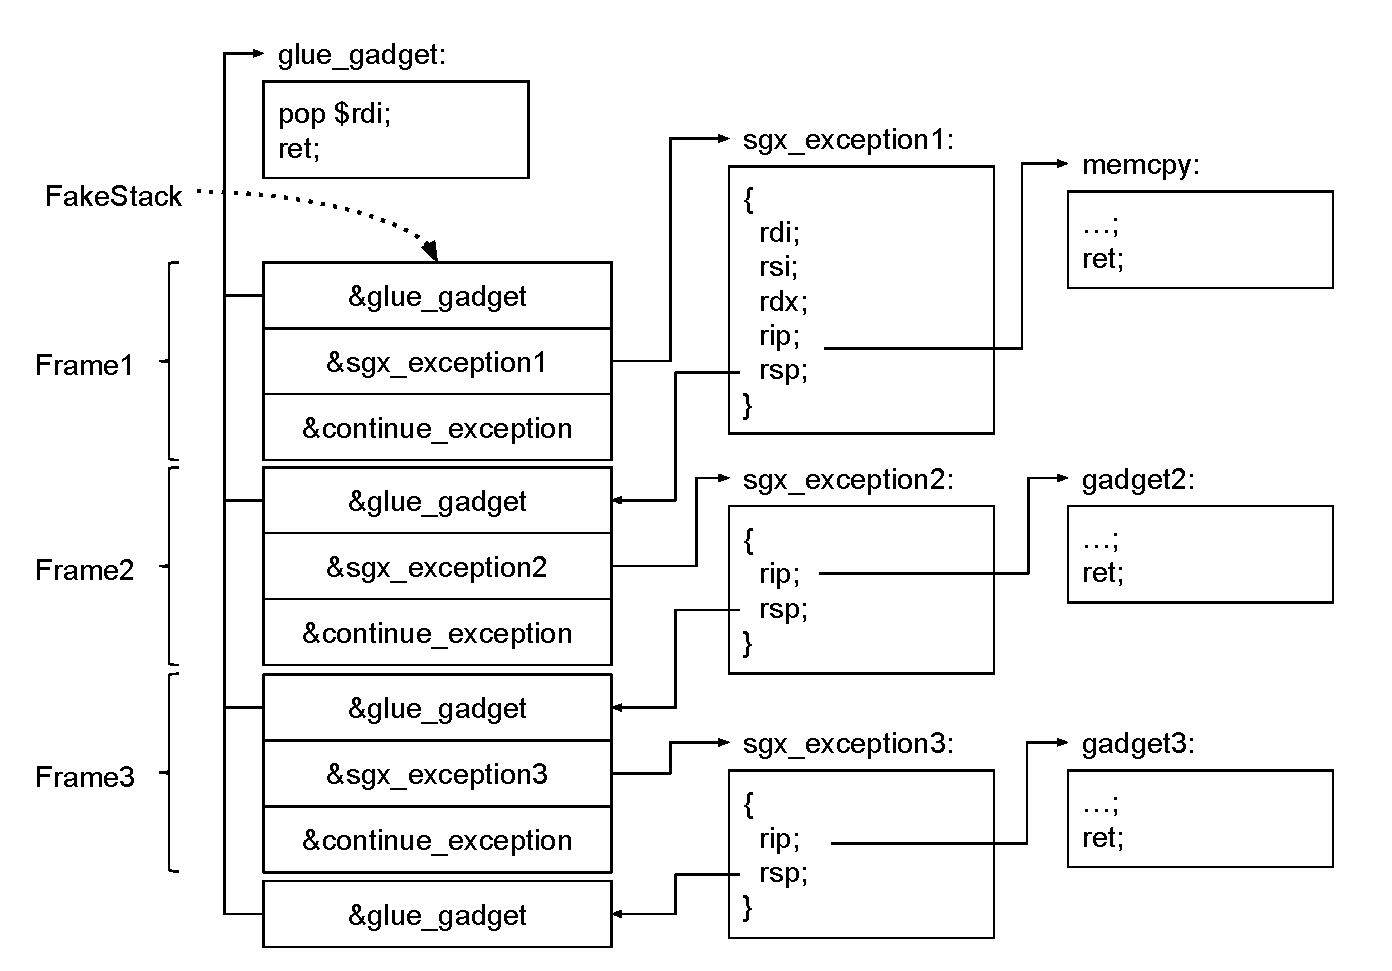
\includegraphics[width=0.8\textwidth]{fig_c5/flavio-enclave-chain.pdf}
	\caption{Chain used in the proof-of-concept of SnakeGX.}
	\label{fig:flavio-enclave-chain}
\end{figure}